\par The Inner Detector~\cite{IDET-2010-01} (ID) is the innermost detector in ATLAS. 
Its two main goals are to track charged particles, some of which are short-lived, 
and to determine their transverse momenta, \pT.
The first goal is achieved by reconstructing data from three sub-detectors that track 
the path of any charged ionizing particle.  
The second goal is achieved by bending the charged particle paths in a 2 T magnetic field 
due to a superconducting solenoid that sorrounds the three aforementioned sub-detectors.
In this setup, the ID is therefore incapable of determining the \pT\ of chargeless particles 
such as photons. The two innermost sub-detectors are 
 the Pixel Detector~\cite{1645094} and the Semiconductor Tracker~\cite{Aad:2014mta} (SCT), which both rely on 
semiconductor technology. The outermost sub-detector is the Transition 
Radiation Tracker~\cite{1748-0221-3-02-P02013} (TRT) and it relies on drift tube technology. 
The 3 sub-detectors are arranged in concentric cylinders around the IP. These cylinders 
are called {\it barrel} components of the sub-detectors. There are also {\it forward} or 
{\it end-cap} components dedicated high-$\eta$ particle tracking. All-in-all
the entire ID structure, including the 2 T solenoid, sits in a \SI{115}{\cm} radius 
cylindrical cavity with a \SI{7}{m} total length in the $z$ direction. The ID components are 
shown in Figure~\ref{fig:wholeID}. 

\begin{figure}
	\centering
   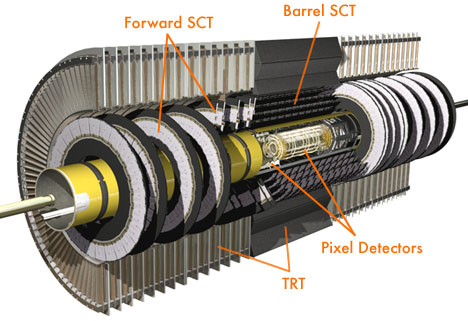
\includegraphics[width=0.8\textwidth]{figures/in_det_lab.jpg}
	\caption{A cutaway view of the ATLAS Inner Detector}
	\label{fig:wholeID}
\end{figure}

\subsubsection{Semiconductor Technology}
\par Semiconductor technology is widely used in modern image capturing devices. A case in point 
is a digital camera sensor, which comprises millions of modular sensors. A sensor of this kind is normally 
made up of a {\it depletion zone} and an electronics readout system. 
A depletion zone is a connective region between two very differently charged regions of 
a semiconductor when a charge equilibrium is achieved; one region is doped with impurities such that there are more free 
electrons than there are positive ions, while the other region is doped such that the 
opposite is true. The connection between these two regions is known as a {\it negative-positive (np) junction}
because of the polar opposite charge populations in the two regions.  
As the free electrons near the np junction  on the n-side 
drift towards the positive ions on the p-side, the region around the junction 
eventually achieves charge equilibrium. When this happens the region is known as the depletion zone, 
and the number of free electrons in the semi-conductor is minimized. 
The depletion zone is therefore a good candidate region for detecting ionizing particles. 

\par In a modern camera sensor, a photon with energy of a few eV deposits all its energy 
in the depletion zone. A bunch of these deposits can knock of enough electrons to form 
a signal, which is amplified and digitized by the electronics readout system of the sensor. Contrastingly, in high 
energy experiments particles with energy of several GeV pass through the depletion zone, ionizing 
the material and leaving a trail of electrons that could be collected as signal. Because of this, 
pixels are used for tracking rather than for energy measurement.

\par The ATLAS Pixel Detector is a good example of a semiconductor detector in high energy physics.
As the sub-detector closest to the IP, it is designed to withstand intense radiation and yet 
provide high resolution precision tracking capabilities. During Run I it was segmented into 
3 barrel layers and 3 end-cap layers, mounted on circular wheels. Expecting higher particle 
rates in Run II, an additional layer called the Insertable B-Layer~\cite{Pohl:2013yda} (IBL) 
was added to become the innermost layer in the barrel. The building block in all these layers 
is the module, which is a group of 46080 pixels sensors. Each pixel in the IBL is     
 $50\times250$~\SI{}{\micron^2} and $50\times400$~\SI{}{\micron^2} everywhere else, 
in $\phi\times z$ in the barrel and $\phi\times r$ in the end-caps.  
The cylindrical arrangement of the modules ensures that the interaction 
point is covered by as much area as possible. This arrangement achieves a spatial 
resolution of $8\times 40$~\SI{}{\micron^2} in the IBL  and $10\times 115$~\SI{}{\micron} 
everywhere else. With 1456 barrel modules and 288 disk modules, 
excluding the IBL, the Pixel Detector covers $|\eta|<2.5$ and $5<r<12$~\SI{}{\cm}. 
The cut-out view of the Pixel Detector in Figure~\ref{fig:pixelD} shows layer segmentation
in both the barrel and end-caps. 

\begin{figure}[!h]
	\centering
   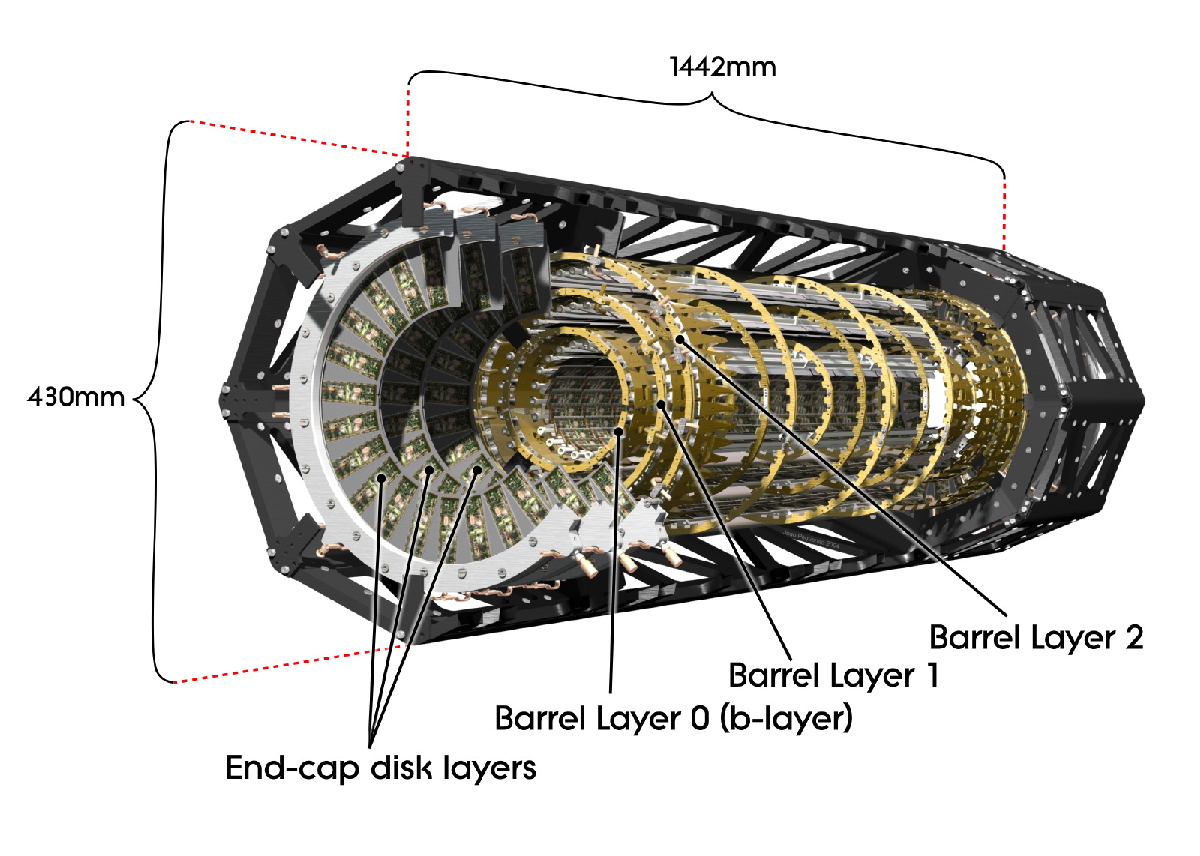
\includegraphics[width=0.8\textwidth]{figures/PixelPerspective.png}
	\caption{A cutaway view of the ATLAS Pixel Detector, which is the innermost sub-detector of the Inner Detector}
	\label{fig:pixelD}
\end{figure}

\par The SCT, which is a cylindrical sub-detector that sits immediately outside 
the Pixel Detector, is another example of a semiconductor detector in ATLAS. 
Covering $30<r<52$~\SI{}{\cm}, a region expected to receive lower particle 
rates than that covered by the Pixel Detector, the SCT affords to use slightly 
less expensive sensors. The sensors in this case are silicon microstrips 
 which are larger than the pixels used in the Pixel Detector.  
Read-out electronics are located on one end of each strip, covering only 
one spatial dimension. To access the second spatial dimension, another microstrip is placed 
at a slight angle to the original strip. The result of this rather forced arrangement is that 
modules in the SCT are different from those in the Pixel Detector. Four strips are laid on 
top of a baseboard used for support. Another set of four perpendicular strips are further laid at 
the bottom of the same baseboard. The crossing between the top and bottom strips covers 
$16\times500$~\SI{}{\micron^2} rectangles. This arrangement achieves a spatial resolution of 
$17\times 580$~\SI{}{\micron^2}. 
While the barrel component of the SCT is made up of 4 layers, the endcap region
 is covered by 9 annular disks on each side, as shown in Figure~\ref{fig:sctD}.
The module arrangement is the same in both regions, covering $|\eta|<2.5$. 

\begin{figure}[!h]
	\centering
   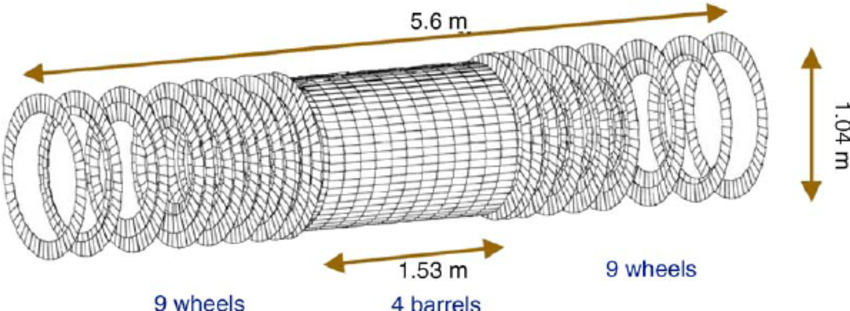
\includegraphics[width=0.8\textwidth]{figures/sct.png}
	\caption{A schematic diagram of the ATLAS SCT}
	\label{fig:sctD}
\end{figure}

\subsubsection{Drift Tube Technology}
\par Drift tube technology is a relatively older technique for detecting ionizing particles
 through a gaseous medium. A more complete discussion of this and other related technologies 
is reserved for Section~\ref{sec:muonSpec}. In a nutshell however, a drift tube is a gas-filled 
cylindrical hollow tube with a thin anode wire on the center and cathode walls. As an ionizing
 particle passes through the gas it liberates electrons 
from atoms, leaving behind positive ions. The electrons drift towards the positive wire at a much greater speed 
than the positive ions do towards the tube walls. The electrons are collected and converted to signal. 

\par The basic sensor for the TRT is a \SI{144}{\cm} long drift tube whose walls are 
made of Kapton, a polymide well known for its stability over a wide range of temperatures, and 
are kept at negative potential. A \SI{30}{\micron} in diameter gold-plated tungsten wire goes through its 
center and is kept at positive potential. The gas in the tube is a mixture 
of 90\% \ch{Xe} , 27\% \ch{CO2} and 3\% \ch{O2}. The \ch{O2} is added to increase electron drift velocity 
towards the tungsten wire and improve the time resolution. 
The TRT barrel region is made up of three identical layers, where each layer is a module. Each layer 
is made up of 32 drift tubes, which are laid parallel to $z$.
The three layers cover a range in $56<r<107$~\SI{}{\cm}, and $|z|< 72$ cm. This corresponds to 
and coverage of $|\eta|<0.7$. The endcap region comprises 18 layers on each side, making up 224 tubes 
on each side, and covering $83<|z|<340$~\SI{}{\cm}. This corresponds to $0.7<|\eta|<2.5$.
The overall resolution achieved with this arrangement is approximately \SI{130}{\micron}.  

%\par Figure~\ref{fig:pieID} shows a comparison of the segmentations in the Pixel, SCT and TRT 
%detectors. 
%
%\begin{figure}[!h]
%	\centering
%   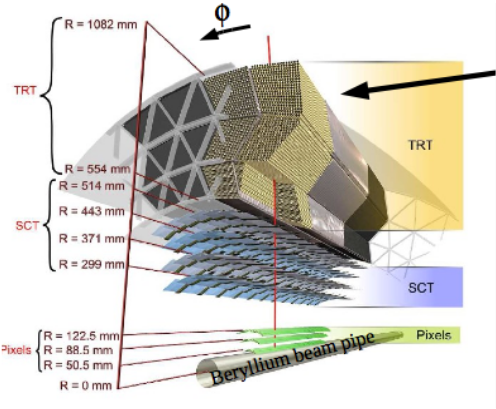
\includegraphics[width=0.8\textwidth]{figures/pieID.png}
%	\caption{Comparison between detector segmentations in the barrel section of the Inner Detector}
%	\label{fig:pieID}
%\end{figure}
